% Select one class
%\documentclass{pucthesis}		% For DVI
% \documentclass[pdftex]{pucthesis}	% For pdfLaTeX
% \documentclass[spanish]{pucthesis}		% For DVI, in spanish
\documentclass[pdftex,spanish]{pucthesis}	% For pdfLaTeX, in spanish

%%%%%%%%% Packages %%%%%%%%%

% Floats
\usepackage{graphicx}
\usepackage{float}
\floatstyle{boxed}
\restylefloat{figure}
\usepackage{subfigure}

% Math packages
\usepackage{amsmath}
\usepackage{amsfonts}
\usepackage{amssymb}

% Closest font to Times New Roman
\usepackage{times}

% To make pretty tables
\usepackage{booktabs}
\usepackage{multirow}

% To avoid underfull errors in the bibliography
\usepackage{etoolbox}
\apptocmd{\sloppy}{\hbadness 10000\relax}{}{}

% To make cites and references
\usepackage[hidelinks,pdfusetitle,pdfdisplaydoctitle]{hyperref}
\usepackage{csquotes}
\usepackage[style=apa,sortcites=true,sorting=nyt,backend=biber]{biblatex}
% \usepackage{doi}
% \renewcommand{\doitext}{}

\usepackage{glossaries}
\makeglossaries
\newglossaryentry{order}{
	name={order},
	description={A request made by a customer through the Pedidos Ya platform for delivery}
}

\newglossaryentry{failrate}{
	name={fail rate},
	description={The percentage of orders that could not be completed due to various reasons}
}

\newglossaryentry{accrate}{
	name={acceptance rate},
	description={The percentage of delivery requests accepted by couriers}
}

\newglossaryentry{blackstores}{
	name={black stores},
	description={Warehouses or fulfillment centers used for fast order processing, typically not open to the public}
}


%--------- NEW ENVIRONMENTS --------- You are free to remove or use it
\newtheorem{definition}{\bf Definition}[chapter]
\newtheorem{property}{Property}[chapter]
\newtheorem{claim}{Claim}[chapter]
\newtheorem{lemma}{\bf Lemma}[chapter]
\newtheorem{proposition}{Proposition}[chapter]
\newtheorem{theorem}{\noindent \bf Theorem}[chapter]
\newtheorem{corollary}{\bf Corollary}[chapter]
\newtheorem{pf}{Proof}[chapter]
\newtheorem{example}{\bf Example}[chapter]
\newtheorem{remark}{Remark}[chapter]

\makeatletter
  \setlength{\beftitle}{105\p@\@plus24\p@}
  \setlength{\afttitle}{65\p@}
\makeatother

\addbibresource{Thesis.bib}

% ----- THEME ----  (Optional)
% Tokyo Night Theme Colors
\usepackage{xcolor}

% Define Tokyo Night color palette
\definecolor{tokyoNightBg}{HTML}{1a1b26}
\definecolor{tokyoNightFg}{HTML}{a9b1d6}
\definecolor{tokyoNightBorder}{HTML}{3d59a1}
\definecolor{tokyoNightBlue}{HTML}{7aa2f7}
\definecolor{tokyoNightCyan}{HTML}{7dcfff}
\definecolor{tokyoNightPurple}{HTML}{bb9af7}
\definecolor{tokyoNightGreen}{HTML}{9ece6a}
\definecolor{tokyoNightRed}{HTML}{f7768e}
\definecolor{tokyoNightOrange}{HTML}{ff9e64}
\definecolor{tokyoNightYellow}{HTML}{e0af68}
\definecolor{tokyoNightComment}{HTML}{565f89}

% Apply theme to document elements
\pagecolor{tokyoNightBg}
\color{tokyoNightFg}

% Hyperlinks styling
\usepackage{hyperref}
\hypersetup{
    colorlinks=true,
    linkcolor=tokyoNightBlue,
    filecolor=tokyoNightGreen,
    urlcolor=tokyoNightCyan,
    citecolor=tokyoNightPurple
}

% Section headings styling
% \usepackage{sectsty}
% \sectionfont{\color{tokyoNightBlue}}
% \subsectionfont{\color{tokyoNightPurple}}
% \subsubsectionfont{\color{tokyoNightCyan}}


% Optional: Code listings with Tokyo Night theme
\usepackage{listings}
\lstset{
    backgroundcolor=\color{tokyoNightBg},
    basicstyle=\color{tokyoNightFg}\ttfamily\small,
    keywordstyle=\color{tokyoNightBlue},
    commentstyle=\color{tokyoNightComment},
    stringstyle=\color{tokyoNightGreen},
    numberstyle=\tiny\color{tokyoNightComment},
    identifierstyle=\color{tokyoNightFg},
    frame=single,
    rulecolor=\color{tokyoNightBorder},
    showstringspaces=false
}
% Table styling
\usepackage{colortbl}

% Bibliography styling
% \usepackage[backend=biber, style=numeric]{biblatex}
% \renewcommand*{\bibfont}{\color{tokyoNightFg}}
% ---- Fin del preambulo ----

\begin{document}
\arrayrulecolor{tokyoNightBorder}

\mdate{Month Day, Year}         % date manuscript changed
\version{1}                                     % manuscript version #

\title[Informe de practica: Pedidos Ya]
{\bf Informe de practica: Pedidos Ya}
\author[Jorge Troncoso Morales]{Jorge Troncoso Morales}

\address{Escuela de Ingenier\'ia\\
{\it Tel.\/} : 56 (2) 354-2000}
\email{jorge.troncoso@alu.ucm.cl}

\facultyto    {the School of Engineering}
%\department   {}
\faculty                {FACULTAD DE INGENIER\'IA}
\degree                  {Master of Science in Engineering}
\advisor                            {Ivan Merino Rodrigez}
\committeememberA {Member A}
\guestmemberA            {Member B}
\ogrsmember                 {Member C}
\subject                            {Structural Engineering}
\date                                 {Marzo 2025}
\copyrightname             {Jorge Troncoso Morales}
\copyrightyear               {MMXV}
% \dedication                      {Gratefully to my parents and siblings}


\NoChapterPageNumber
\pagenumbering{roman}
\maketitle


%\newpage
%\thispagestyle{empty}

%%%%%%%%%%%%%%%%%%
%          page v & up ---                      %
%            Table of contents              %
%            List of figures                     %
%            List of tables                      %
%%%%%%%%%%%%%%%%%%

\pdfbookmark{\contentsname}{toc}
\tableofcontents
\phantomsection \label{listoffigures}
\listoffigures
\phantomsection \label{listoftables}
\listoftables
\cleardoublepage

%%%%%%%%%%%%% TEXT  OF THESIS %%%%%%%%%%%%%

\pagenumbering{arabic}
\chapter[DESCRIPCION GENERAL DE LA EMPRESA]{descripcion general de la empresa}
PedidosYa es una empresa líder en la industria de delivery online en América Latina, especializada en la intermediación entre comercios y clientes a través de su plataforma digital. Fundada en 2009 en Uruguay, la compañía ha experimentado un crecimiento exponencial y actualmente opera en múltiples países de la región, incluyendo Argentina, Chile, México, Brasil y Colombia, entre otros.

La empresa forma parte del grupo Delivery Hero \parencite{deliveryhero_pedidosya2025}, una de las mayores compañías de entrega de alimentos y productos a nivel global. Su plataforma permite a los usuarios acceder a una amplia variedad de servicios, desde la compra de alimentos en restaurantes hasta la entrega de productos de supermercados, farmacias y tiendas especializadas.

PedidosYa se distingue por su enfoque en la tecnología y la optimización logística, ofreciendo una experiencia de usuario eficiente a través de su aplicación móvil y sitio web. La empresa utiliza algoritmos avanzados para mejorar los tiempos de entrega, optimizar las rutas de los repartidores y brindar opciones de pago seguras y flexibles.

Además de su core business en food delivery, PedidosYa ha expandido su portafolio con servicios como PedidosYa Market, un modelo de dark stores que permite entregas ultrarrápidas de productos de conveniencia, y PedidosYa Envíos, que ofrece soluciones logísticas para empresas y usuarios particulares \parencite{pedidosya_envios}.

Con una cultura empresarial dinámica y orientada a la innovación, PedidosYa continúa evolucionando dentro del ecosistema de comercio electrónico y delivery, adaptándose a las nuevas demandas del mercado y consolidándose como un actor clave en la transformación digital del sector.


\chapter[ROLES Y RESPONSABILIDADES DE LA PRACTICA]{Roles y responsabilidades de la practica} \label{ch1}
\section{Descripción General de la Posición: Courier Business Intern \label{sec:sec1}}
El rol de \textit{Courier Business Intern} consiste en apoyar las labores del área de Courier Business, participando activamente en tareas de análisis de datos, operaciones y business intelligence. Este puesto complementa el trabajo del Sr. Analyst, colaborando en la recolección, análisis y presentación de información, así como en la implementación de soluciones operativas específicas para PedidosYa Envíos.

\section{Responsabilidades Clave \label{sec:sec2}}
Aunque el enfoque principal del rol es el análisis de datos y la toma de decisiones basadas en información, las responsabilidades se llevan a cabo en coordinación con el equipo de Courier Business. Es importante señalar que PedidosYa cuenta con equipos especializados (BI, Operaciones y Logística) para abordar estos desafíos de forma integral; sin embargo, para tareas y problemas específicos, se requiere una solución más focalizada dentro del equipo de Courier Business.

\subsection{Análisis de Datos y Reporte}
\begin{itemize}
  \item \textbf{Recolección y Procesamiento de Datos:} Extraer y organizar datos relevantes para evaluar el desempeño de las operaciones.
  \item \textbf{Búsqueda de Insights:} Identificar tendencias y oportunidades de mejora a partir de los datos analizados.
  \item \textbf{Generación y Presentación de Reportes:} Elaborar informes detallados que respalden la toma de decisiones estratégicas, en colaboración con el Sr. Analyst.
\end{itemize}

\subsection{Soporte en Operaciones}
\begin{itemize}
  \item \textbf{Tareas Operativas Específicas:} Realizar actividades no críticas como renombrar partners, activar cuentas o gestionar partners no clave (Key Accounts).
  \item \textbf{Implementación de Soluciones:} Colaborar en la aplicación de mejoras operativas que requieran un enfoque personalizado y granular.
\end{itemize}

\subsection{Presentación y Toma de Decisiones}
\begin{itemize}
  \item \textbf{Reuniones Semanales:} Preparar y exponer semanalmente reportes e insights ante el equipo y el Manager.
  \item \textbf{Sugerencias Estratégicas:} Proponer recomendaciones basadas en los análisis realizados para optimizar las operaciones y procesos.
\end{itemize}

\section{Herramientas y Tecnologías Utilizadas \label{sec:sec3}}
Para llevar a cabo las tareas descritas, PedidosYa utiliza diversas soluciones tecnológicas que facilitan la gestión de datos y la comunicación interna. Entre las principales herramientas se encuentran:

\begin{enumerate}
  \item \textbf{Jira:} Sistema de gestión de tickets utilizado para el escalado de incidencias de clientes y agentes.\footnote{Más información en: \url{https://www.atlassian.com/software/jira}}
  \item \textbf{Slack:} Plataforma de comunicación interna que permite una interacción fluida entre miembros de diferentes equipos.\footnote{Más información en: \url{https://slack.com/}}
  \item \textbf{Google Cloud Platform (GCP):} Infraestructura para la gestión de recursos tecnológicos y de datos.\footnote{Más información en: \url{https://cloud.google.com/gcp}}
  \item \textbf{BigQuery:} Servicio de almacenamiento y gestión de bases de datos SQL, parte de GCP, que facilita la extracción y análisis de información.\footnote{Más información en: \url{https://cloud.google.com/bigquery}}
  \item \textbf{Locker Studio:} Herramienta integrada en GCP para la creación de dashboards y consultas simples.
  \item \textbf{JupyterHub:} Plataforma IDE en línea para escribir código, principalmente en Python, utilizando librerías como Pandas y Matplotlib para la manipulación y visualización de datos.\footnote{Más información en: \url{https://jupyter.org/hub}}
  \item \textbf{Google Spreadsheets:} Aplicación similar a Excel para la creación de hojas de cálculo y tablas dinámicas, con funcionalidades de colaboración en tiempo real.\footnote{Más información en: \url{https://www.google.com/sheets/about/}}
\end{enumerate}




\chapter[PROYECTOS Y TAREAS]{Proyectos y tareas} \label{ch2}
\section{Tareas}
\subsection{Revision de casos Jira}
Pedidos Ya cuenta con un sistema de tickets dirigido tanto a clientes (B2B) como a consumidores (C2B). El servicio de PedidosYa Envios opera en ambos segmentos, por lo que se solicita frecuentemente el contacto con agentes de servicio para resolver incidencias en las órdenes. Para atender estos casos se sigue un Procedimiento Operativo Estándar (SOP) que define las acciones a seguir; sin embargo, cuando se presentan situaciones ambiguas, el caso se escala directamente al equipo de Courier para su revisión.

Esta tarea, una de las más rutinarias realizadas, consistía en revisar el historial de \textit{chat} acompañado de imágenes para comprender la situación. Se trataba de una gestión operativa enfocada en determinar si las órdenes fallidas (Fail Rate) debían ser compensadas o denegadas, requiriendo mayor criterio y objetividad que desafíos técnicos.

Es importante señalar que, aunque esta tarea es rutinaria y no implica una responsabilidad crítica, una gestión inadecuada podría generar fricción con consumidores o clientes B2B. Además, esta actividad se llevó a cabo durante las primeras tres semanas del internado, para posteriormente ser transferida a un equipo especializado en la sede central de Uruguay.

\subsection{Analisis de datos}

El area Courier de PedidosYa suele trabajar con KPI's similares a los de PedidosYa en general, como pueden ser:

\begin{itemize}
	\item Fail Rate \eqref{eq:FR}: Para medir la tasa de ordenes que no suelen ser exitosas. \textbf{Se busca reducir.}

	      \begin{equation} \label{eq:FR}
		      \text{Fail Rate} = \frac{\text{Rejected Orders}}{\text{Total Orders}} \times 100\%
	      \end{equation}

	\item Acceptance Rate \eqref{eq:AR}: Cuando una orden es emitida, se envia una notifiacion a los repartidores o \textit{Riders}, dicha orden puede ser aceptada o rechazada. El Acceptance Rate mide la tasa con la que los repartidores aceptan las ordenes. \textbf{Se busca aumentar.}
	      \begin{equation} \label{eq:AR}
		      \text{Acceptance Rate} = \frac{\text{Riders Accept}}{\text{Riders Notified}} \times 100\%
	      \end{equation}
	\item Vendor Late \eqref{eq:VL}: Una orden tiene varias fases desde que se emite la orden hasta que es entregada por el rider, uno de los mas importantes es el Vendor Late, el cual mide el tiempo que pasa desde el que el Rider llega al local y se le es entregada la orden. \textbf{Se busca reducir.}
	      \begin{equation}\label{eq:VL}
		      \text{Vendor Late} = \text{Pick up datetime} - \text{Rider Arrival datetime}
	      \end{equation}
\end{itemize}

Una vez comprendido los principales KPI's del negocio, fue necesario estudiar los datos de los que dispone PedidosYa. Estos suelen estar alojados en BigQuery, por lo que para acceder a ellos se debio hacer mediante permisos y la ejecucion de \textit{Queries} en usando SQL.

El Fail Rate suele estar sujeto a un monton de causas, para no relevar exactamente cuales son las problematicas afectan PedidosYa Envios, se usaran nombre genericos. El dataset usado en tareas rutinarias de analisis de datos tenia siguientes campos:

\begin{table}[htbp]
\caption{Dataset de órdenes registradas}
  \raggedright
	\label{tab:main_dataset}
	\begin{threeparttable}
		\begin{tabular}{lc}
			\toprule
			\textbf{Field}         & \textbf{Datatype} \\
			\midrule
			order\_id              & Integer           \\
			partner\_id            & Integer           \\
			date                   & Datetime          \\
			status\_BO             & String            \\
			partner                & String            \\
			partner\_or\_franchise & String            \\
			reason\_text           & String            \\
			globalCode             & Integer           \\
			declared\_value        & Float             \\
			\bottomrule
		\end{tabular}
		\begin{tablenotes}[para]
			\small
			\textit{Nota.} Los tipos de datos son presentados de forma genérica.
		\end{tablenotes}
	\end{threeparttable}
\end{table}

Este dataset es una pesudo tabla de hechos, que contiene el registro de todos las ordenes realizadas. La query para este dataset generalmente solo se limitaba para traer las ordenes del mes.
\subsection{Presentacion semanal de insights}
\section{Proyectos}
\subsection{Presentacion para clientes B2B}


\chapter[REFLECCIONES Y LECCIONES APRENDIDAS]{Reflecciones y lecciones aprendidas} \label{ch3}
\section{Aprendizaje}

Durante el período de práctica, adquirí y reforcé tanto habilidades técnicas como blandas. Gran parte de este aprendizaje fue posible gracias al equipo de Courier cuyo apoyo, paciencia y disposición para explicar tanto aspectos del negocio como herramientas utilizadas fueron fundamentales. Además, sus experiencias y conocimientos compartidos fueron valiosos y los considero un gran aporte para mi desarrollo profesional.

Uno de los aprendizajes más significativos fue comprender en profundidad el entorno laboral real enfrentándome a problemáticas concretas, responsabilidades en la toma de decisiones y la necesidad de una comunicación clara y efectiva. Aprendí a sintetizar información técnica de manera asertiva y accesible un aspecto clave en cualquier entorno empresarial. Asimismo, experimenté de primera mano la importancia de una buena dinámica de equipo y cómo la colaboración efectiva impacta en los resultados.

En cuanto a habilidades técnicas, adquirí conocimientos tanto en \textbf{análisis de datos} como en \textbf{negocios}. Estar presente en reuniones entre managers de distintas áreas y observar cómo los Account Managers negociaban con clientes me permitió comprender mejor el funcionamiento estratégico de la empresa. A nivel técnico, fortalecí mis conocimientos en \textbf{estadística y programación}, y entendí en profundidad la relevancia de \textbf{SQL} y las consultas avanzadas para la recopilación y análisis de datos.

\section{Oportunidades de mejora}

Desde el punto de vista de la experiencia profesional, la práctica fue altamente enriquecedora. El ambiente de trabajo fue exigente pero gratificante, y la empresa mantuvo un equilibrio entre el aprendizaje y la autonomía en las tareas asignadas. Además, la gestión por parte de la universidad para acceder a la práctica fue ágil y eficiente.

Si tuviera que mencionar un área de mejora, sería la falta de una guía previa que ayudara a los practicantes a anticipar ciertos aspectos relevantes para la elaboración del informe final. Por ejemplo, PedidosYa mantiene un alto nivel de confidencialidad respecto a sus datos y operaciones, lo que implicó restricciones estrictas en el acceso y manejo de información. Se me asignó un computador de la empresa con normas específicas para prevenir vulnerabilidades y filtraciones, lo que significó que no pude extraer información directamente para este informe. Aunque existía la posibilidad de tomar fotografías a la pantalla, decidí no hacerlo, ya que me parecía poco profesional y una práctica que podría interpretarse como una vulneración de las políticas de seguridad de la empresa.

Contar con una guía o una orientación previa sobre estas restricciones habría sido útil para planificar mejor la recopilación de información necesaria para el informe, dentro de los márgenes permitidos. No obstante, esta situación también me permitió desarrollar una mayor \textbf{conciencia sobre la gestión de datos sensibles} y la importancia de respetar las normativas empresariales en entornos corporativos.



\chapter[CONCLUSIONSES]{Conclusionses}
La experiencia en PedidosYa Envios marcó un antes y un después en mi desarrollo profesional y personal, permitiéndome aplicar y ampliar los conocimientos adquiridos en la carrera de Ingeniería Industrial. Durante mi práctica, tuve la oportunidad de enfrentar desafíos reales en un entorno laboral dinámico, lo que me impulsó a perfeccionar tanto mis habilidades técnicas como mis competencias interpersonales.

A lo largo de este periodo, comprendí la importancia de utilizar herramientas tecnológicas, como SQL, BigQuery y la Suite de Google, para transformar datos en insights que apoyen la toma de decisiones estratégicas. Este proceso no solo mejoró mi capacidad analítica, sino que también fortaleció mi compromiso con la precisión y la eficiencia en el manejo de la información.

Por otra parte, la experiencia me enseñó el valor de una comunicación clara y concisa en contextos colaborativos. La interacción con equipos multidisciplinarios y la participación en reuniones estratégicas me permitieron desarrollar la habilidad de presentar resultados y recomendaciones de forma accesible y orientada a objetivos comunes. Asimismo, me familiaricé con la realidad de operar bajo restricciones de seguridad y confidencialidad, lo que reforzó mi respeto por las buenas prácticas en la gestión de datos.

En definitiva, la práctica profesional en PedidosYa Envios no solo potenció mis competencias técnicas, sino que también me proporcionó una visión integral del funcionamiento de un negocio B2B en el sector logístico. Esta experiencia ha consolidado mi vocación y me ha preparado para enfrentar futuros desafíos con mayor seguridad y responsabilidad, constituyéndose como un pilar fundamental en mi formación profesional y personal.




%%%%%%%%%%%%% REFERENCES %%%%%%%%%%%%%

\cleardoublepage
\phantomsection \label{references}
\renewcommand{\bibname}{REFERENCIAS}

%%%% ACTIVAR SIGUIENTES 3 LINEAS SI POSTGRADO RECHAZA LA BIBLIOGRAFIA
%\setlength{\bibleftmargin}{0em}
%\setlength{\bibindent}{0em}
%\setlength{\bibitemsep}{1em}


\printbibliography

%%%%%%%%%%%% APPENDICES %%%%%%%%%%%%

\appendix
\chapter[First Appendix]{First Appendix}
\begin{figure}[h!] % Or other placement options like t, b, p
\begin{flushleft}
  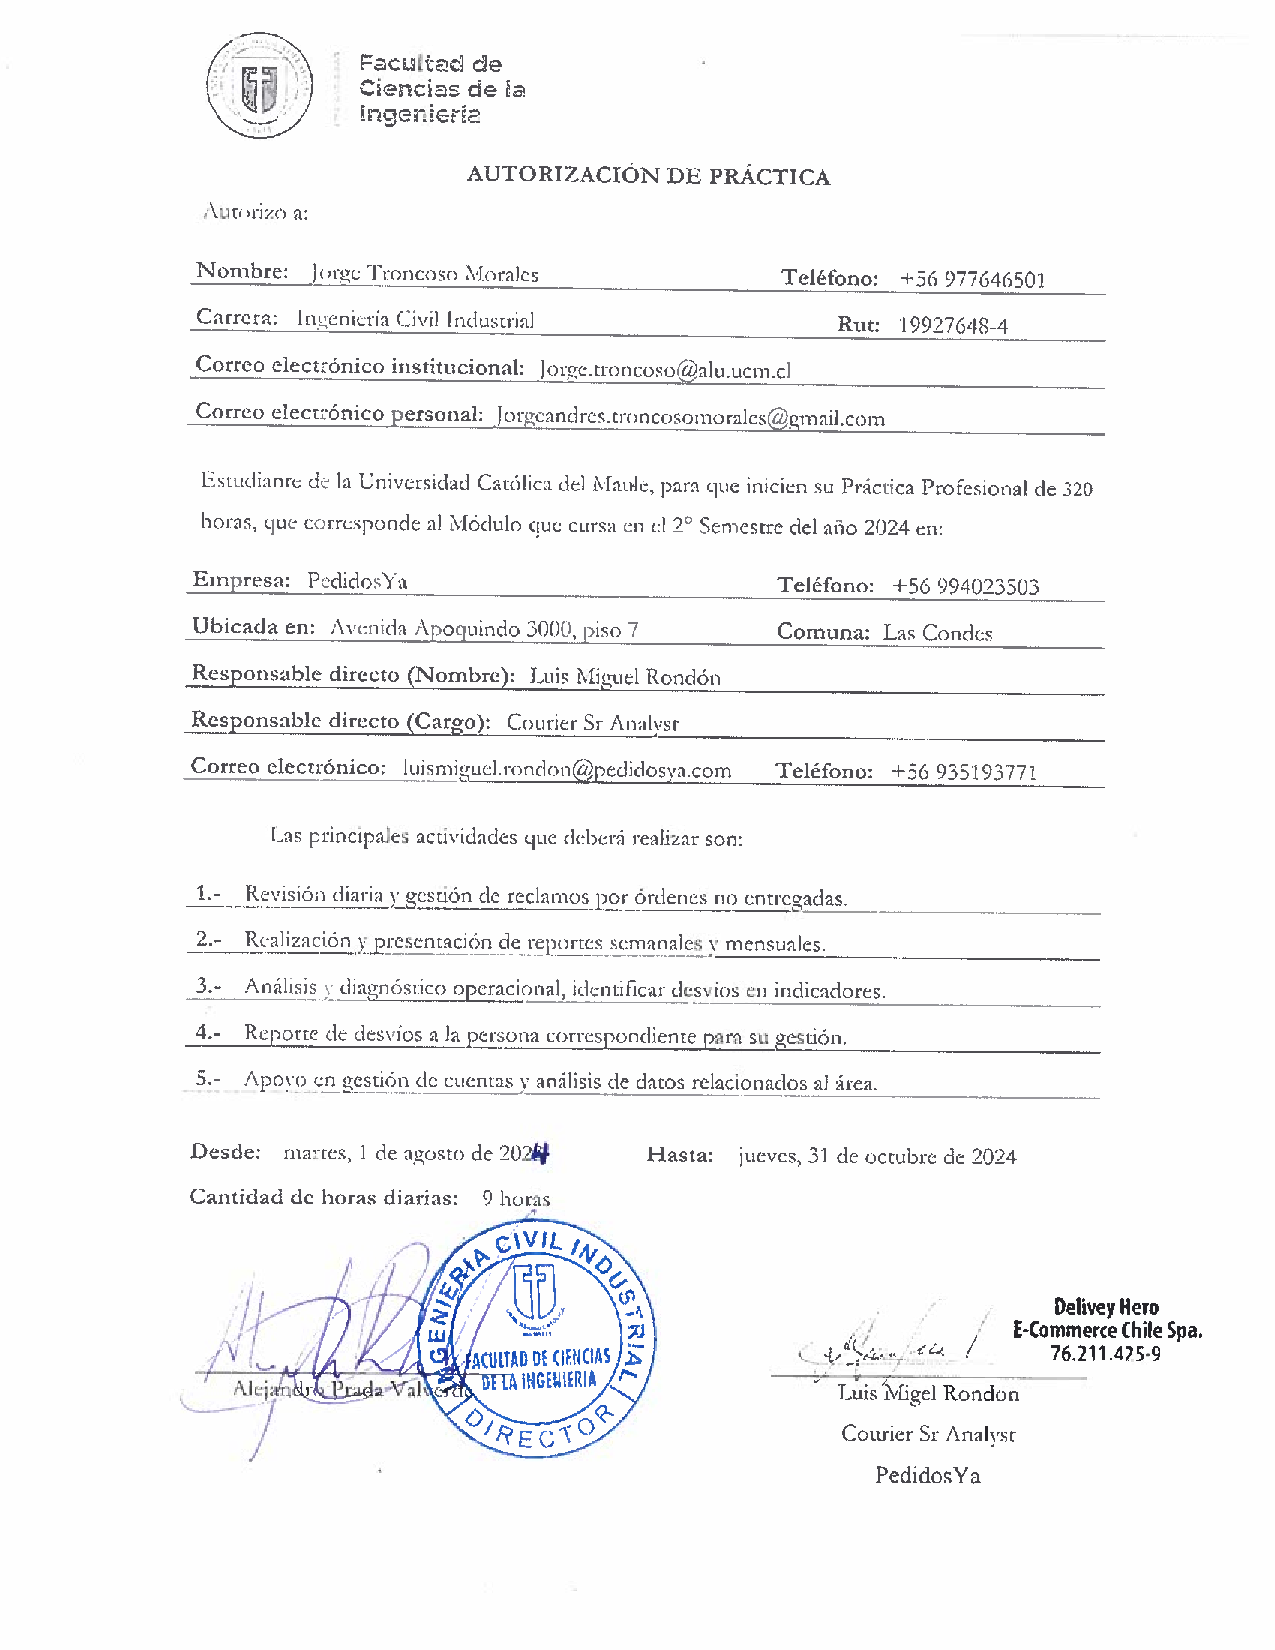
\includegraphics[width=\linewidth]{figures/autorizacion_practica.pdf}
\end{flushleft}
\caption{Autorizacion de practica en PedidosYa}
\label{fig: autorizacion_practica}
\end{figure}


\end{document}
